\chapter{Results}\label{ch:results}

\section{Use}
Members made 71\,460 trips. By Equation~\eqref{eq:use} this is
\[
  u = \frac{71\,460}{120 \times 182} \approx 3.3
\]
trips per bicycle per day, above the target of 2.5. Figure~\ref{fig:trips} shows average daily trips by month. Weekday use rose steadily until May, dipped in June and July when teaching stopped, and reached its highest level in August as students returned. Weekend use grew in every month.

\begin{figure}[htbp]
  \centering
  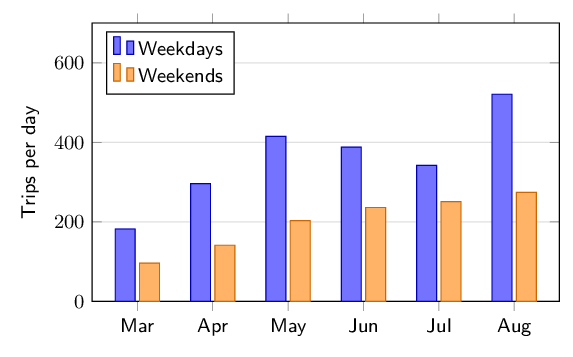
\includegraphics[width=0.75\textwidth]{figures/daily-trips.png}
  \caption{Average trips per day by month, for weekdays and weekends.}
  \label{fig:trips}
\end{figure}

Use was uneven between stations, as Table~\ref{tab:stations} shows. The Library and the railway station together accounted for 42\% of all trips, while Sports Centre and East Gate accounted for 7\%.

\begin{table}[htbp]
  \centering
  \caption{Trips starting at each station over the pilot.}
  \label{tab:stations}
  \begin{tabular}{lrr}
    \toprule
    Station & Trips & Share (\%) \\
    \midrule
    Library            & 16\,150 & 22.6 \\
    Railway station    & 13\,862 & 19.4 \\
    Northgate          & 11\,720 & 16.4 \\
    Science Quarter    & 10\,290 & 14.4 \\
    Students' Union    &  8\,504 & 11.9 \\
    Main Building      &  5\,932 &  8.3 \\
    Sports Centre      &  2\,858 &  4.0 \\
    East Gate          &  2\,144 &  3.0 \\
    \midrule
    Total              & 71\,460 & 100.0 \\
    \bottomrule
  \end{tabular}
\end{table}

\section{Cost}
Table~\ref{tab:cost} sets out income and costs. By Equation~\eqref{eq:cost} the net cost was 2.10 per trip, below the target of 2.50.

\begin{table}[htbp]
  \centering
  \caption{Operating cost and income over the pilot.}
  \label{tab:cost}
  \begin{tabular}{lr}
    \toprule
    Item & Amount \\
    \midrule
    Operator's fee            & 132\,000 \\
    Maintenance and repairs   &  31\,400 \\
    Staff time                &  23\,960 \\
    \midrule
    Total operating cost      & 187\,360 \\
    Membership income         &  37\,294 \\
    \midrule
    Net cost                  & 150\,066 \\
    Net cost per trip         &     2.10 \\
    \bottomrule
  \end{tabular}
\end{table}

\section{Effect on Car Travel}
Of the 412 survey respondents, 58 (14\%) said that their most recent trip would otherwise have been made by car, as driver or passenger. A further 201 (49\%) would have walked, 117 (28\%) would have taken a bus and 36 (9\%) would not have made the trip. The 14\% figure meets the target of 10\%. Because people who responded may differ from those who did not, we treat it as an estimate with a margin of roughly three percentage points either way.

\section{Summary Against the Goals}
All three goals in Section~\ref{sec:goals} were met: 3.3 trips per bicycle per day against a target of 2.5, a net cost of 2.10 per trip against 2.50, and 14\% of trips replacing a car journey against 10\%.
